\documentclass[a4paper,11pt,dvipdfmx]{jsarticle}

\usepackage[margin=25mm]{geometry}
\usepackage{array}
\usepackage{longtable}
\usepackage{booktabs}
\usepackage[dvipdfmx]{graphicx}
\usepackage[dvipdfmx]{hyperref}
\usepackage{url}

\hypersetup{
  colorlinks=true,
  urlcolor=blue
}

\title{『トポロジー最適化入門』正誤表}
\author{矢地謙太郎}
\date{最終更新：\today}

\begin{document}

\maketitle

本書に関する誤植・訂正事項を以下にまとめます．
ご指摘いただいた皆様に感謝申し上げます．

\vspace{1em}

\setlength{\tabcolsep}{5pt}
\renewcommand{\arraystretch}{1.15}

\begin{longtable}{
@{}
>{\centering\arraybackslash}m{0.06\textwidth}
>{\raggedright\arraybackslash}m{0.13\textwidth}
>{\centering\arraybackslash}m{0.365\textwidth}
>{\centering\arraybackslash}m{0.365\textwidth}
@{}
}

\toprule
頁 & 箇所 & 誤 & 正 \\
\midrule
\endfirsthead

\toprule
頁 & 箇所 & 誤 & 正 \\
\midrule
\endhead

36 &
図2.12(a) &
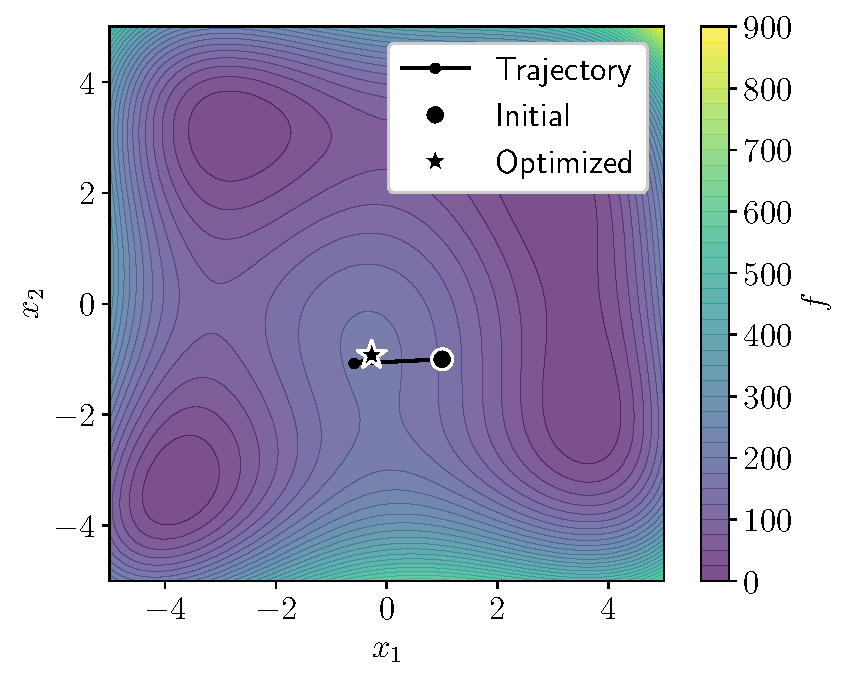
\includegraphics[width=0.95\linewidth]{fig/ch02_212_a_f.pdf} &
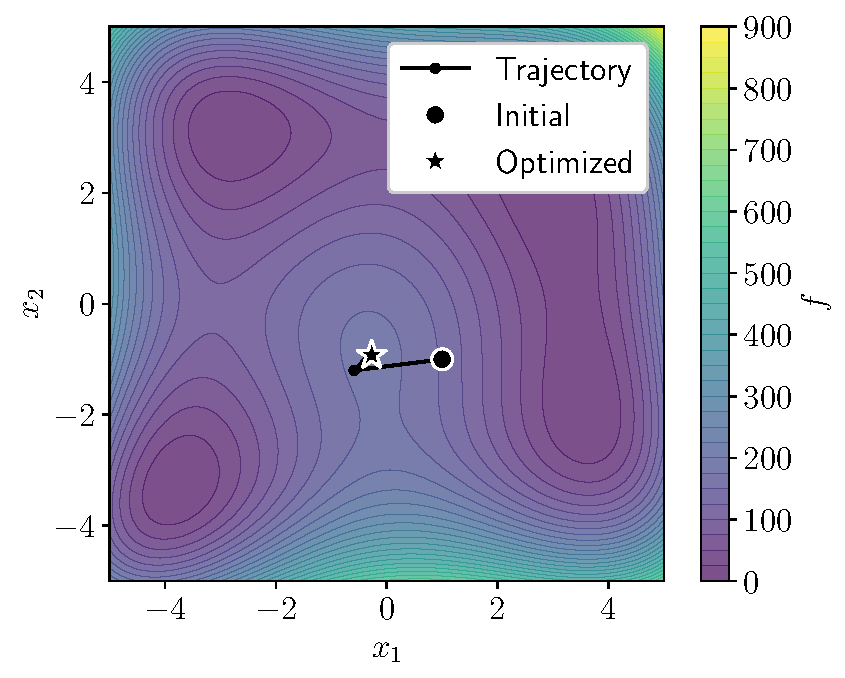
\includegraphics[width=0.95\linewidth]{fig/ch02_212_a_t.pdf}
\\[1ex]

\multicolumn{4}{@{}p{0.97\textwidth}@{}}{%
\small
\textbf{訂正内容：}
Pythonコード(\href{https://github.com/yajiken0609/topology-optimization-book/blob/master/ch02.ipynb}{\texttt{ch02.ipynb}})上で，ヘッセ行列の対角成分
\texttt{8*x[0]} は，正しくは
\texttt{8*x[0]**2} です．
これを修正すると，収束の軌跡が少し変化します．
\hfill{\footnotesize （第1刷）}
}
\\[1.5ex]

%=================================================================
\midrule
123 &
図2.12(b) &
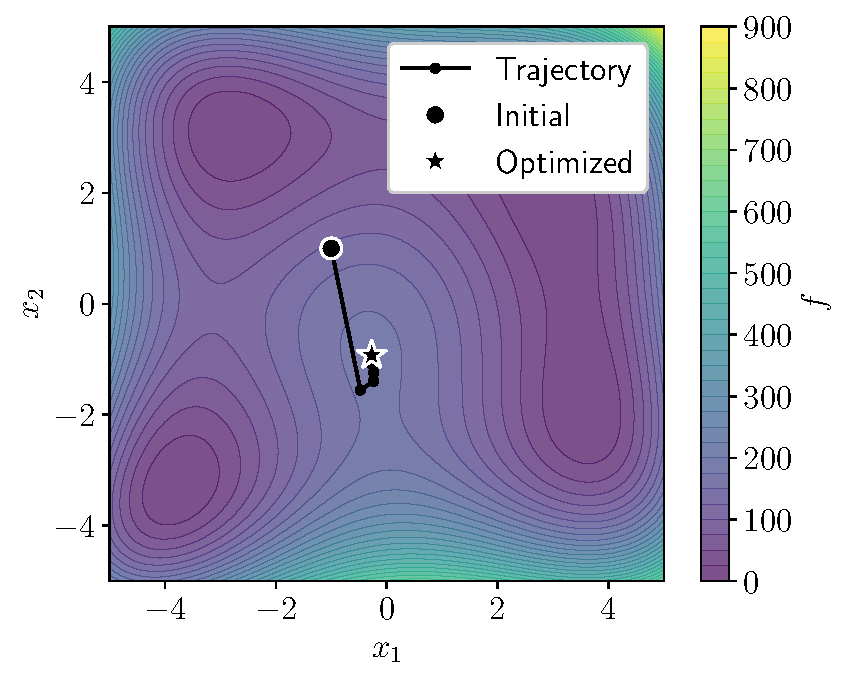
\includegraphics[width=0.95\linewidth]{fig/ch02_212_b_f.pdf} &
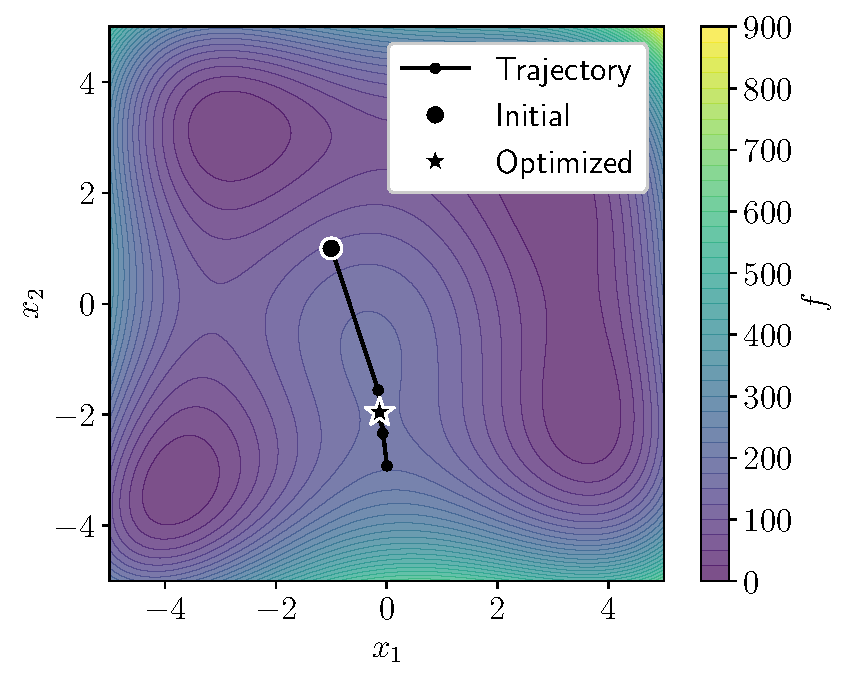
\includegraphics[width=0.95\linewidth]{fig/ch02_212_b_t.pdf}
\\[1ex]

\multicolumn{4}{@{}p{0.97\textwidth}@{}}{%
\small
\textbf{訂正内容：}
同上．
\hfill{\footnotesize （第1刷）}
}
\\[1.5ex]
%=================================================================

\bottomrule
\end{longtable}

\vfill

\noindent
最新版のPythonコードは以下で公開しています．\\
\url{https://github.com/yajiken0609/topology-optimization-book}

\end{document}
